\newsavebox{\smlmat}
\savebox{\smlmat}{$\smm{1&1\\1&0}$}
\newsavebox{\smlmatb}
\savebox{\smlmatb}{$\smm{1&1\\1&1}$}
\newsavebox{\smlmatc}
\savebox{\smlmatc}{$\smm{1&1&1\\0&1&0}$}

\section{Characterizations}
\begin{obs}
Let $P\in\Pat$ and $P'\in\{0,1\}^{k\times l+1}$ such that $P'=P\oplus_h0^{k\times1}$, similarly let $M\in\Mat$ and $M'\in\{0,1\}^{m\times n+1}$ such that $M'=M\oplus_h0^{m\times1}$, then $\PimM\Leftrightarrow P'\im M'$.
\end{obs}
\begin{proof}
\begin{itemize}
\item[$\Rightarrow$] Clearly we can map the last column of $P'$ to the last column of $M'$ and then map (using OR) $P'[[k],[l]]$ to $M'[[m],[n]]$ the same way $P$ is mapped to $M$.
\item[$\Leftarrow$] If $P'\im M$ we are done. Otherwise, the last column of $P'$ needs to be mapped to the last column of $M'$ and by deleting both from their matrix we get $P'[[k],[l]]\im M'[[m],[n]]$ which is the same as $\PimM$.
\end{itemize}
\end{proof}

The same proof can be also used for adding an empty column as the first column or an empty row as the first or the last row. Using induction we can easily show that a pattern $P'$ is avoided by a matrix $M'$ if and only if $P$ is avoided by $M$ where $P$ is derived from $P'$ by excluding all empty beginning or ending rows and columns and $M$ is derived from $M'$ by excluding the same number of beginning or ending rows and columns. Therefore, when characterizing matrices avoiding a forbidden pattern, we do not need to consider patterns having empty rows or columns on their boundary.

\begin{defn}
A \emph{walk} in a matrix~$M$ is a sequence of some of its entries, beginning in the top left corner and ending in the bottom right one. If an entry $M[i,j]$ is in the sequence, the next one is either $M[i+1,j]$ or $M[i,j+1]$.
\end{defn}
\begin{defn}
We call a binary matrix~$M$ a \emph{walking matrix} if there is a walk in $M$ such that all one-entries of $M$ are contained on the walk.
\end{defn}
\begin{defn}
An \emph{extended walk of size $k\times l$} in a matrix~$M$ is a subset of some of its entries, beginning in the top left corner and ending in the bottom right one. If an entry $M[i,j]$ is in the subset there is also either $M[i+1,j]$ or $M[i,j+1]$. The size describes that no more than $k$ entries directly above each other are in the subset and no more than $l$ entries directly next to each other are in the subset. We say that an extended walk of size $k\times l$ in $M$ starts with a walk~$w$, if the extended walk is a subset of entries of $M$ that
\begin{itemize}
\item lie on $w$ or below $w$ and
\item lie on $w$ shifted by $k-1$ down and by $l-1$ to the left or above it.
\end{itemize}
\end{defn}
\begin{defn}
For $M\in\Mat$ and $r\in[m],c\in[n]$ we say $M[r,c]$ is
\begin{itemize}
\item \emph{top-left empty} if $M[[r-1],[c-1]]$ is an empty matrix,
\item \emph{top-right empty} if $M[[r-1],[c+1,n]]$ is empty,
\item \emph{bottom-left empty} if $M[[r-1],[c+1,n]]$ is empty,
\item \emph{bottom-right empty} if $M[[r-1],[c+1,n]]$ is empty.
\end{itemize}
\end{defn}
\subsection{Patterns of size $2\times2$ and their generalization}
\begin{thm}
Let $P=\smm{0&1\\1&0}$, then for all $M$: $\PnimM\Leftrightarrow M$ is a walking matrix.
\end{thm}
\begin{proof}
Since $P$ is a permutation matrix, $\PnimM\Leftrightarrow\PnsmM$ and it is easy to see $\PnsmM\Leftrightarrow M$ is a walking matrix.
\end{proof}

Now consider a generalization of the pattern from above:
\begin{thm}
Let $P\in\Pat$ be a matrix having only two one-entries -- $P[1,n]$ and $P[m,1]$, then for all $M$: $\PnimM\Leftrightarrow M$ has an extended walk of size $k-1\times l-1$ containing all one-entries.
\end{thm}
\begin{proof}
\begin{itemize}
\item[$\Rightarrow$] Let $\PnimM$ and consider the left-most top-right empty elements of $M$. They necessarily form a walk $w$. For contradiction, assume there is a one-entry $e$ below the extended walk of size $k-1\times l-1$ starting with $w$. Since $e$ is below the extended walk, there is an element $e'$ - the right-most element of $M$ that is neither below $e$ nor to the right from $e$ and at the same time still below the extended walk (it is possible $e=e'$). Let $e=M[r,c]$ and notice $M[r-k,c-l]$ is part of walk $w$ and because of the choice of $e'$ neither $M[r-k-1,c-l]$ nor $M[r-k,c-l-1]$ are on the walk $w$ and $M[r-k,c-l]$ must be a one-entry; therefore, together with $e$ it forms the forbidden pattern in $M$, which is a contradiction.
\item[$\Leftarrow$] Let $M[r,c]$ be any one-entry of $M$, which then necessarily lie in the extended walk. Because the size of the walk is $k-1\times l-1$, $M[r-k+1,c-l+1]$ is top-left empty and $M[r+k-1,c+l-1]$ is bottom-right empty; therefore $e$ cannot be a part of a mapping of $P$. 
\end{itemize}
\end{proof}

\begin{thm}
\label{theorem1}
Let $P=\smm{1&1\\1&0}$, then for all $M\in\Mat$: $\PnimM\Leftrightarrow$ there exist a row~$r$ and a column~$c$ such that (see Figure~\ref{p12})
\begin{itemize}
\item $M[[r-1],[c-1]]$ is empty,
\item $M[[r-1],[c+1,n]]$ is empty,
\item $M[[r+1,m],[c-1]]$ is empty and
\item $M[[r,m],[c,n]]$ is a walking matrix.
\end{itemize}
\end{thm}
\begin{figure}[h!]
\centering
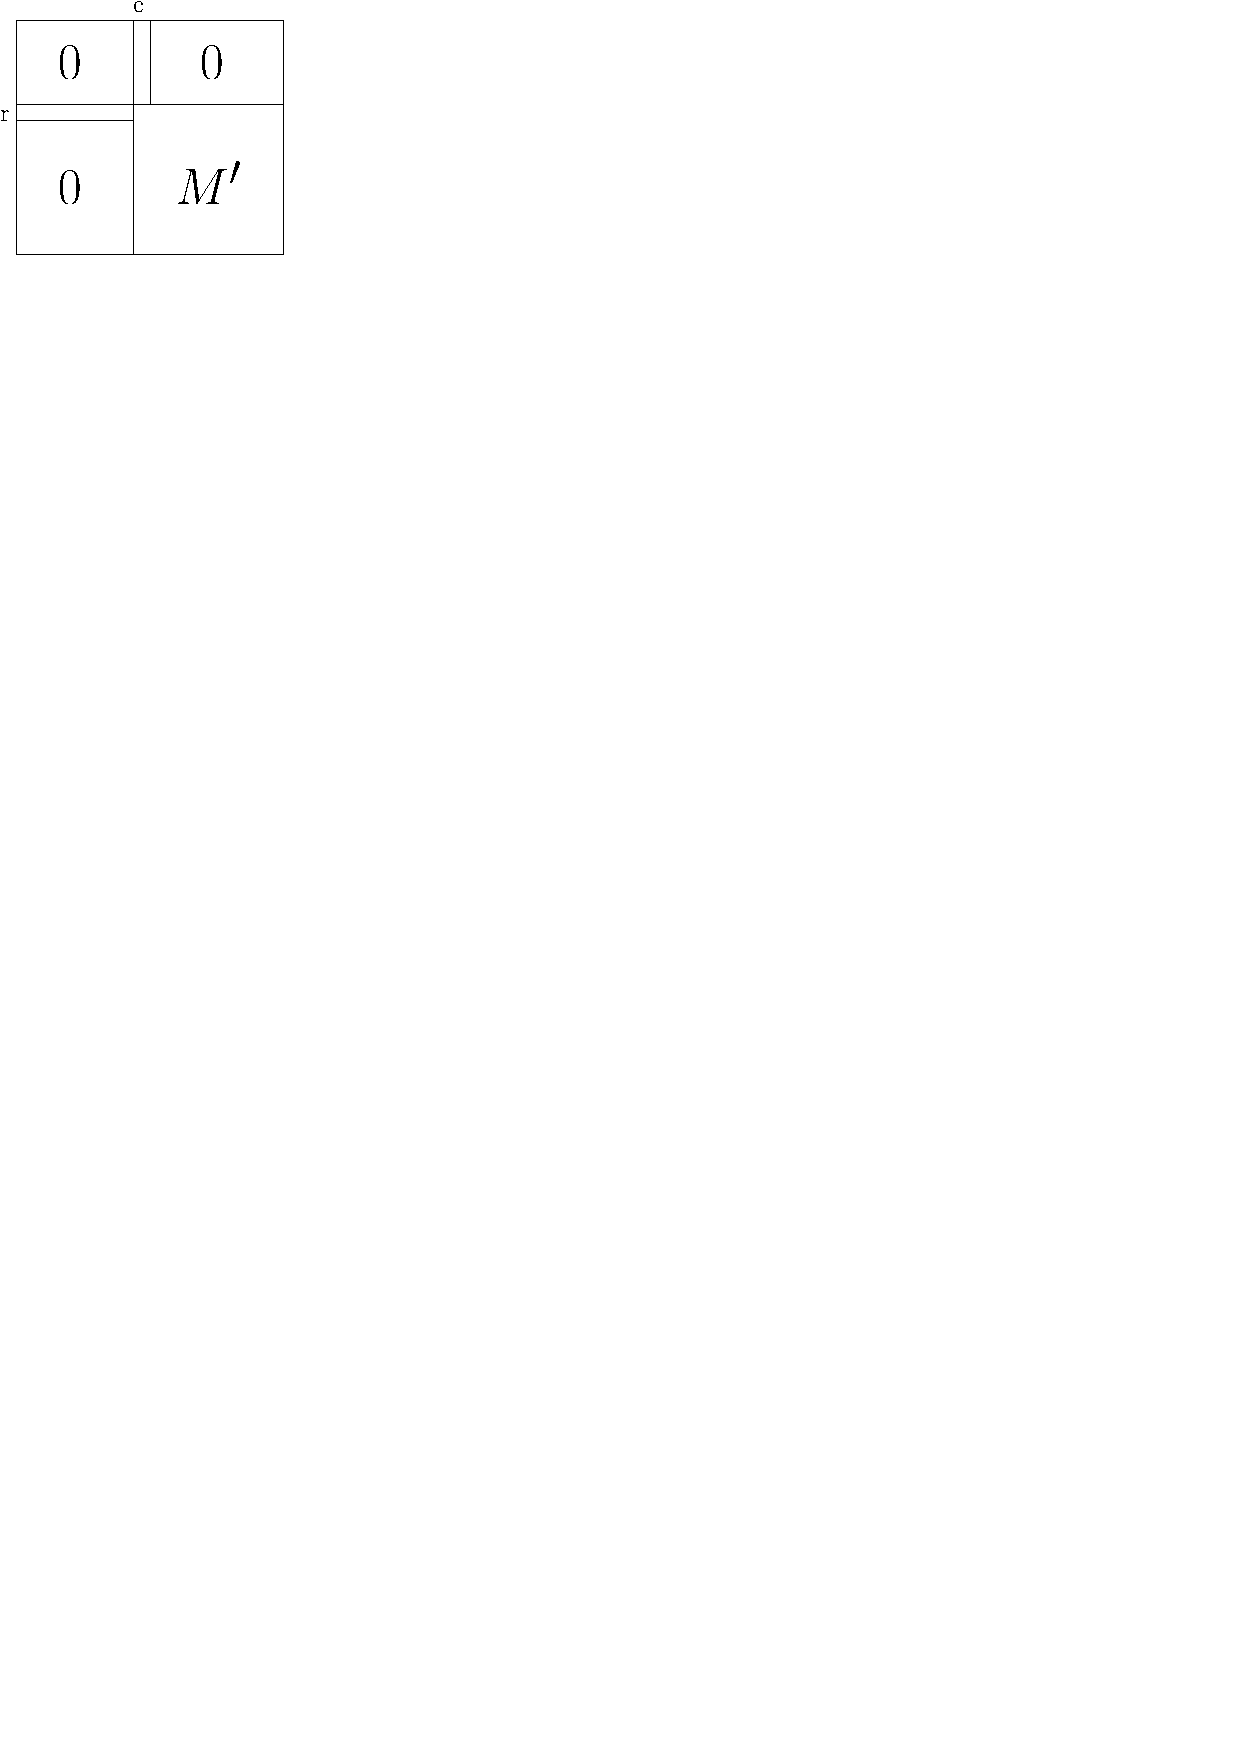
\includegraphics[width=60mm]{img/p12.pdf}
\caption{Characterization of a matrix avoiding \usebox{\smlmat} as an interval minor. Matrix $M'$ is a walking matrix}
\label{p12}
\end{figure}
\begin{proof}
\begin{itemize}
\item[$\Rightarrow$] If $\smm{0&1\\1&0}\nim M$ then $M$ is a walking matrix and we set $r=c=1$. Otherwise, there are one-entries $M[r,c']$ and $M[r',c]$ such that $r'<r$ and $c'<c$. If there is a one-entry in regions $M[[r-1],[c-1]],\ M[[r-1],\ [c+1,n]]$ or $M[[r+1,m],[c-1]]$ then $\PimM$. If $M[[r,m],[c,n]]$ is not a walking matrix then it contains $\smm{0&1\\1&0}$ and we again get a contradiction.
\item[$\Leftarrow$] For contradiction, assume that $M$ described in Figure~\ref{p12} contains $P$ as an interval minor. It means that there is a partition of the matrix into four quadrants such that there is at least one one-entry in each quadrant besides the bottom right one. If the matrix is partitioned above the $r$-th row, then there is only one column containing one-entries and it is not possible for both top quadrants to have a one-entry. Similarly, if the matrix is partitioned to the left of the $c$-th column, there is only one row containing one-entries and there is no one-entry in either top-left or bottom-left quadrant. Therefore, the partitioning lies bellow the $r$-th row and to the right of the $c$-th column, but if the quadrants contain one-entries, there is a $\smm{0&1\\1&0}$ interval minor in $M'$, which is a contradiction with it being a walking matrix. % there has to be a way to write this better
\end{itemize}
\end{proof}

\begin{thm}
Let $P\in\Pat$ be a matrix having only three one-entries -- $P[1,1],\ P[1,n]$ and $P[m,1]$, then for all $M$: $\PnimM\Leftrightarrow$ there exist a row~$r$ and a column~$c$ such that (see Figure~\ref{p12} and imagine rows and columns being extended)
\begin{itemize}
\item $M[[r-1],[c-1]]$ is empty,
\item $M[[r-1],[c+l,n]]$ is empty,
\item $M[[r+k,m],[c-1]]$ is empty and
\item $M[[r,m],[c,n]]$ has an extended walk of size $k-1\times l-1$ containing all one-entries.
\end{itemize}
\end{thm}
\begin{proof} Let $P'=P$ and set $P'[m,1]=0$ ($P'$ is a generalization of $\smm{0&1\\1&0}$). 
\begin{itemize}
\item[$\Rightarrow$] If $P'\nim M$ then $M$ is a matrix having an extended walk of size $k-1\times l-1$ containing all one-entries and we set $r=c=1$. Otherwise, there are one-entries $M[r_1,c_1]$ and $M[r_2,c_2]$ such that $r_2<r_1$ and $c_1<c_2$. We now choose $M[r_3,c_3]$ to be the bottom-most one-entry that still forms $P'$ with $M[r_2,c_2]$. We choose $M[r_4,c_4]$ to be the left-most one-entry that forms $P'$ with $M[r_3,c_3]$ and set $r=r_3-k+1$ and $c=c_4-l+1$. If there is a one-entry in regions $M[[r-1],[c-1]],\ M[[r-1],\ [c+l,n]]$ or $M[[r+k,m],[c-1]]$ then $\PimM$. If $M[[r,m],[c,n]]$ is not a walking matrix then it contains $P'$ and we again get a contradiction.
\item[$\Leftarrow$] Because of the sizes of areas with no one-entries and the condition for $M[[r,m],[c,n]]$, there cannot be $P'$ anywhere but in $M[[r+k-1],[c+l-1]]$. Since $M[[r-1][c-1]]$ is empty, there is no one-entry to map $P[1,1]$ to; therefore, $\PnimM$.
\end{itemize}
\end{proof}

\begin{lemma}
\label{lemma1}
Let $P=\smm{1&1\\1&1}$ and let $M\in\Mat$ avoid $P$ as an interval minor, then there exists a row~$r$ and a column~$c$ such that $M[r,c]$ is either
\begin{enumerate}
\item a one-entry and $(r,c)\in\{(1,1),(1,n),(m,1),(m,n)\}$ or
\item both top-left empty and bottom-right empty and $(r,c)\not\in\{(1,n),(m,1)\}$ or
\item both top-right empty and bottom-left empty and $(r,c)\not\in\{(1,1),(m,n)\}$.
\end{enumerate}
\end{lemma}
\begin{proof}
If there is a one-entry in any corner we are done. Otherwise, let $A$ be a set of all top-left empty entries of $M$ and $B$ be a set of all bottom-right empty entries of $M$. If there is an entry $M[r,c]\in A\cap B$ different from $(1,n)$ and $(m,1)$ we are done. Assume $A\cap B=\{(1,n),(m,1)\}$. Since $(m,1)\in A$, it also holds $(m-1,1)\in A$ and because it is not in the intersection we have $(m-1,1)\not\in B$. This means $M[m-1,1]$ is not bottom-right empty; therefore there is a one-entry somewhere in $M[{m},[2,n]]$. Moreover, no corner contains a one-entry so the is a one-entry in $M[{m},[2,n-1]]$. For simplicity, we will say that the last row in non-empty (knowing the corners are empty). Symmetrically, we also get that the first row is non-empty and both the first and the last columns are non-empty. If there is a one-entry $M[r_l,1]$ in a different row than a one-entry $M[r_r,n]$ and at the same time a one-entry $M[1,c_t]$ in a different column than a one-entry $M[m,c_b]$ then these four one-entries form a mapping of the forbidden pattern $P$.

This is not true!!!
%% the last statement is not true -- need to fix it, there is one more case and symmetry - will use a picture to deal with it

Without loss of generality assume there is only one one-entry in both the first and the last column and they are both in the same row $r'$. Let $c'$ be a column such that there is a one-entry $M[1,c']$. Clearly, there is no other column that contains a one-entry above $r'$, because we would again get a contradiction. Symmetrically, let $c''$ be the only column containing one-entries below $r'$. If $c'\geq c''$ we have that both $M[r',c']$ and $M[r',c'']$ are both top-left empty and bottom-right empty, which is a contradiction with $A\cap B=\{(1,n),(m,1)\}$. Otherwise, $c'<c''$ and both $M[r',c']$ and $M[r',c'']$ are both top-right empty and bottom-left empty where $(r',c')\not\in\{(1,1),(m,n)\}$ which concludes the proof.
\end{proof}

\begin{thm}
Let $P=\smm{1&1\\1&1}$, then for all $M$: $\PnimM\Leftrightarrow M$ looks like one of the matrices in Figure~\ref{p33}, where $\smm{1&1\\1&0}\nim M_1$, $\smm{0&1\\1&1}\nim M_2$, $\smm{1&1\\0&1}\nim M_3$ and $\smm{1&0\\1&1}\nim M_4$.
\end{thm}
\begin{figure}[h!]
\centering
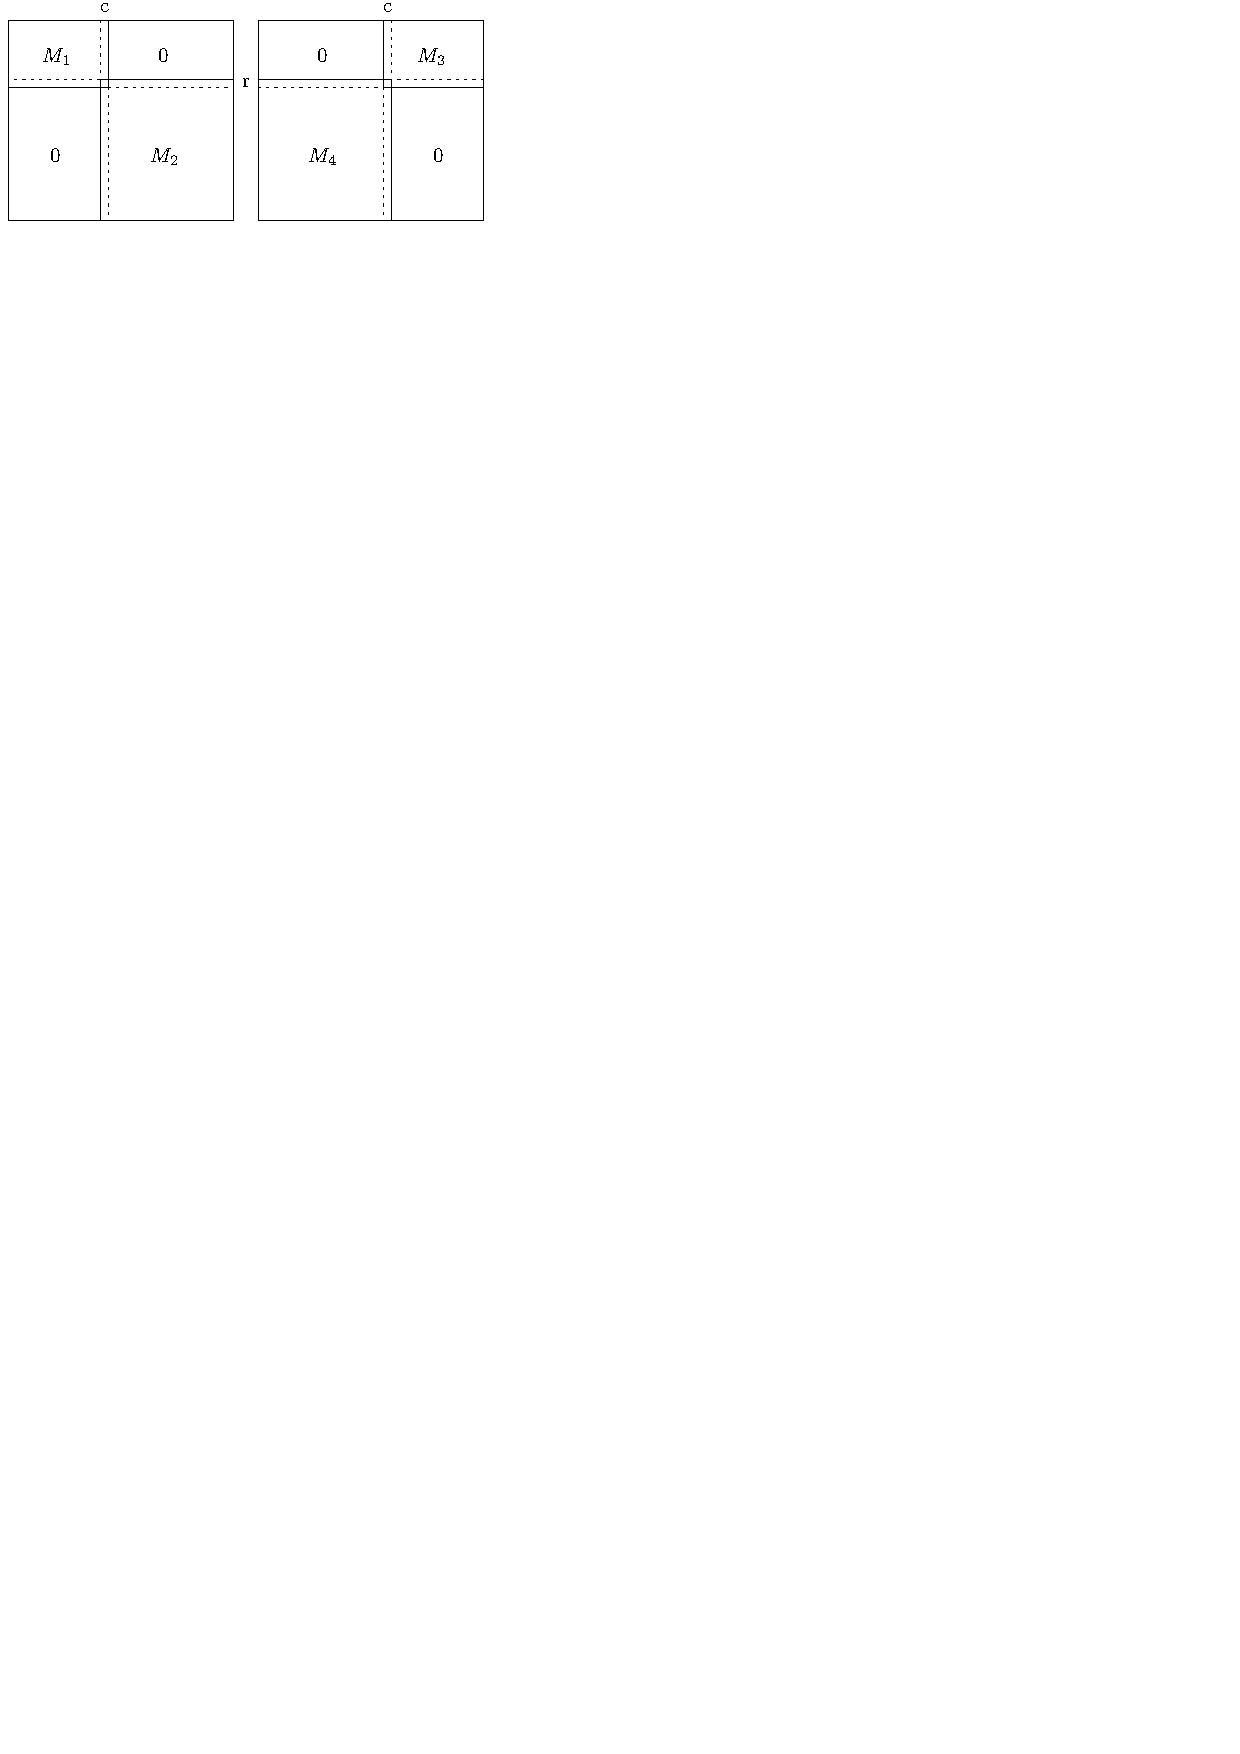
\includegraphics[height=60mm]{img/p33.pdf}
\caption{Characterization of a matrix avoiding \usebox{\smlmatb} as an interval minor.}
\label{p33}
\end{figure}
\begin{proof}
\item[$\Rightarrow$] We proceed by induction by the size of $M$.

If $M\in\{0,1\}^{2\times2}$ then it either avoids $\smm{0&1\\1&1}$ or $\smm{1&1\\1&0}$ and we are done.

For bigger $M$ there is, from Lemma~\ref{lemma1}, $M[r,c]$ satisfying some conditions. If it is the first condition -- there is a one-entry in any corner, we are done because the matrix cannot contain one of the rotations of $\smm{1&1\\1&0}$. Assume the second case -- $M[r,c]$ is both top-right and bottom-left empty and $(r,c)\not\in\{(1,n),(m,1)\}$. If $M_1$ is non-empty, then $\smm{0&1\\1&1}\nim M_2$; otherwise, $\PimM$. Similarly, $\smm{1&1\\1&0}\nim M_1$ if $M_2$ is non-empty. If one of them is empty, the other is a smaller matrix avoiding $P$ as an interval minor and by induction hypothesis, it can be partitioned. Adding empty rows and columns does not break any condition and we get a partitioning of the whole $M$.
\item[$\Leftarrow$] Without loss of generality, let us assume $M$ looks like the left matrix in Figure~\ref{p33}. For contradiction, assume $\PimM$. In that case, we can partition $M$ into four quadrants such that there is at least one one-entry in each of them. It does not matter where we partition it, every time we either get $\smm{1&1\\1&0}\im M_1$ or $\smm{0&1\\1&1}\im M_2$, which is a contradiction.
\end{proof}

\begin{thm}
Let $P\in\Pat$ be a matrix having only four one-entries -- $P[1,1],\ P[1,n],\ P[m,1]$ and $P[m,n]$, then for all $M$: $\PnimM\Leftrightarrow M$ looks like one of the matrices in Figure~\ref{p33}, where generalized $\smm{1&1\\1&0}\nim M_1$, $\smm{0&1\\1&1}\nim M_2$, $\smm{1&1\\0&1}\nim M_3$ and $\smm{1&0\\1&1}\nim M_4$.
\end{thm}
% a lot to do here - probably will need a generalization of the lemma1

\subsection{Matrices of size $2\times3$}
\begin{thm}
Let $P=\smm{1&0&1\\0&1&0}$, then for all $M$: $\PnimM\Leftrightarrow M=M_1\oplus_hM_2$ where $\smm{1&0\\0&1}\nim M_1$ and $\smm{0&1\\1&0}\nim M_2$.
\end{thm}
\begin{proof}
\begin{itemize}
\item[$\Rightarrow$] Let $e=[r,c]$ be the top-most one-entry of $M$. If $\smm{1&0\\0&1}\im M[[m],[c-1]]$, together with $e$ it forms $P$. If $\smm{0&1\\1&0}\nim M[[m],[c,n]]$ then we are done. Let us assume it is not the case and let $e_{0,0},\ e_{1,1}$ be any two one-entries forming the forbidden pattern. Symmetrically, let $\smm{1&0\\0&1}\im M[[m],[c]]$ and let $e_{0,1},\ e_{1,0}$ be any two one-entries forming the forbidden pattern. Now if we take $e_{0,0},\ e_{0,1}$ and $e_{1,0}$ or $e_{1,1}$ with bigger row, we get the forbidden pattern $P$ as an interval minor of $M$. 
\item[$\Leftarrow$] For contradiction, let us assume $\PimM$ and $M=M_1\oplus_hM_2$. If $\PimM$, look at the one-entry of $M$ where the bottom one-entry of $P$ is mapped. If it is in $M_1$ then $\PnimM$ because $\smm{0&1\\1&0}\nim M_1$. Otherwise, $\PnimM$ because $\smm{1&0\\0&1}\nim M_2$.
\end{itemize}
\end{proof}
\begin{lemma}
\label{lemma2}
Let $P=\smm{1&1&1\\0&1&0}$, then for all $M$: $\PnimM\Rightarrow M=M_1\oplus_hM_2$ where
\begin{enumerate}
\item $\smm{1&1\\0&1}\nim M_1$ and $\smm{0&1\\1&0}\nim M_2$ or
\item $\smm{1&0\\0&1}\nim M_1$ and $\smm{1&1\\1&0}\nim M_2$.
\end{enumerate}
\end{lemma}
\begin{proof}
Let $e=[r,c]$ be the top-most one-entry of $M$. If $\smm{1&1\\0&1}\im M[[m],[c-1]]$, together with $e$ it would be the whole $P$. Similarly, $\smm{1&1\\1&0}\nim M[[m],[c+1,n]]$. For contradiction with the statement, let $\smm{1&0\\0&1}\im M[[m],[c]]$ and $e_{0,0},\ e_{1,1}$ (none of them equal to $e$, since $e$ lies in the top-right corner) be any two one-entries forming the pattern. Symmetrically, let $\smm{0&1\\1&0}\im M[[m],[c,n]]$ and $e_{0,1},\ e_{1,0}$ be any two one-entries forming the pattern. In that case $e_{0,0},\ e,\ e_{0,1}$ and $e_{1,0}$ or $e_{1,1}$ with bigger row give us the forbidden pattern $P$ as an interval minor of $M$.
\end{proof}
\begin{thm}
Let $P=\smm{1&1&1\\0&1&0}$, then for all $M$: $\PnimM\Leftrightarrow M$ looks like the matrix in Figure~\ref{p72} and $\smm{1&0\\0&1}\nim M_1$ and $\smm{0&1\\1&0}\nim M_2$.
\end{thm}
\begin{figure}[h!]
\centering
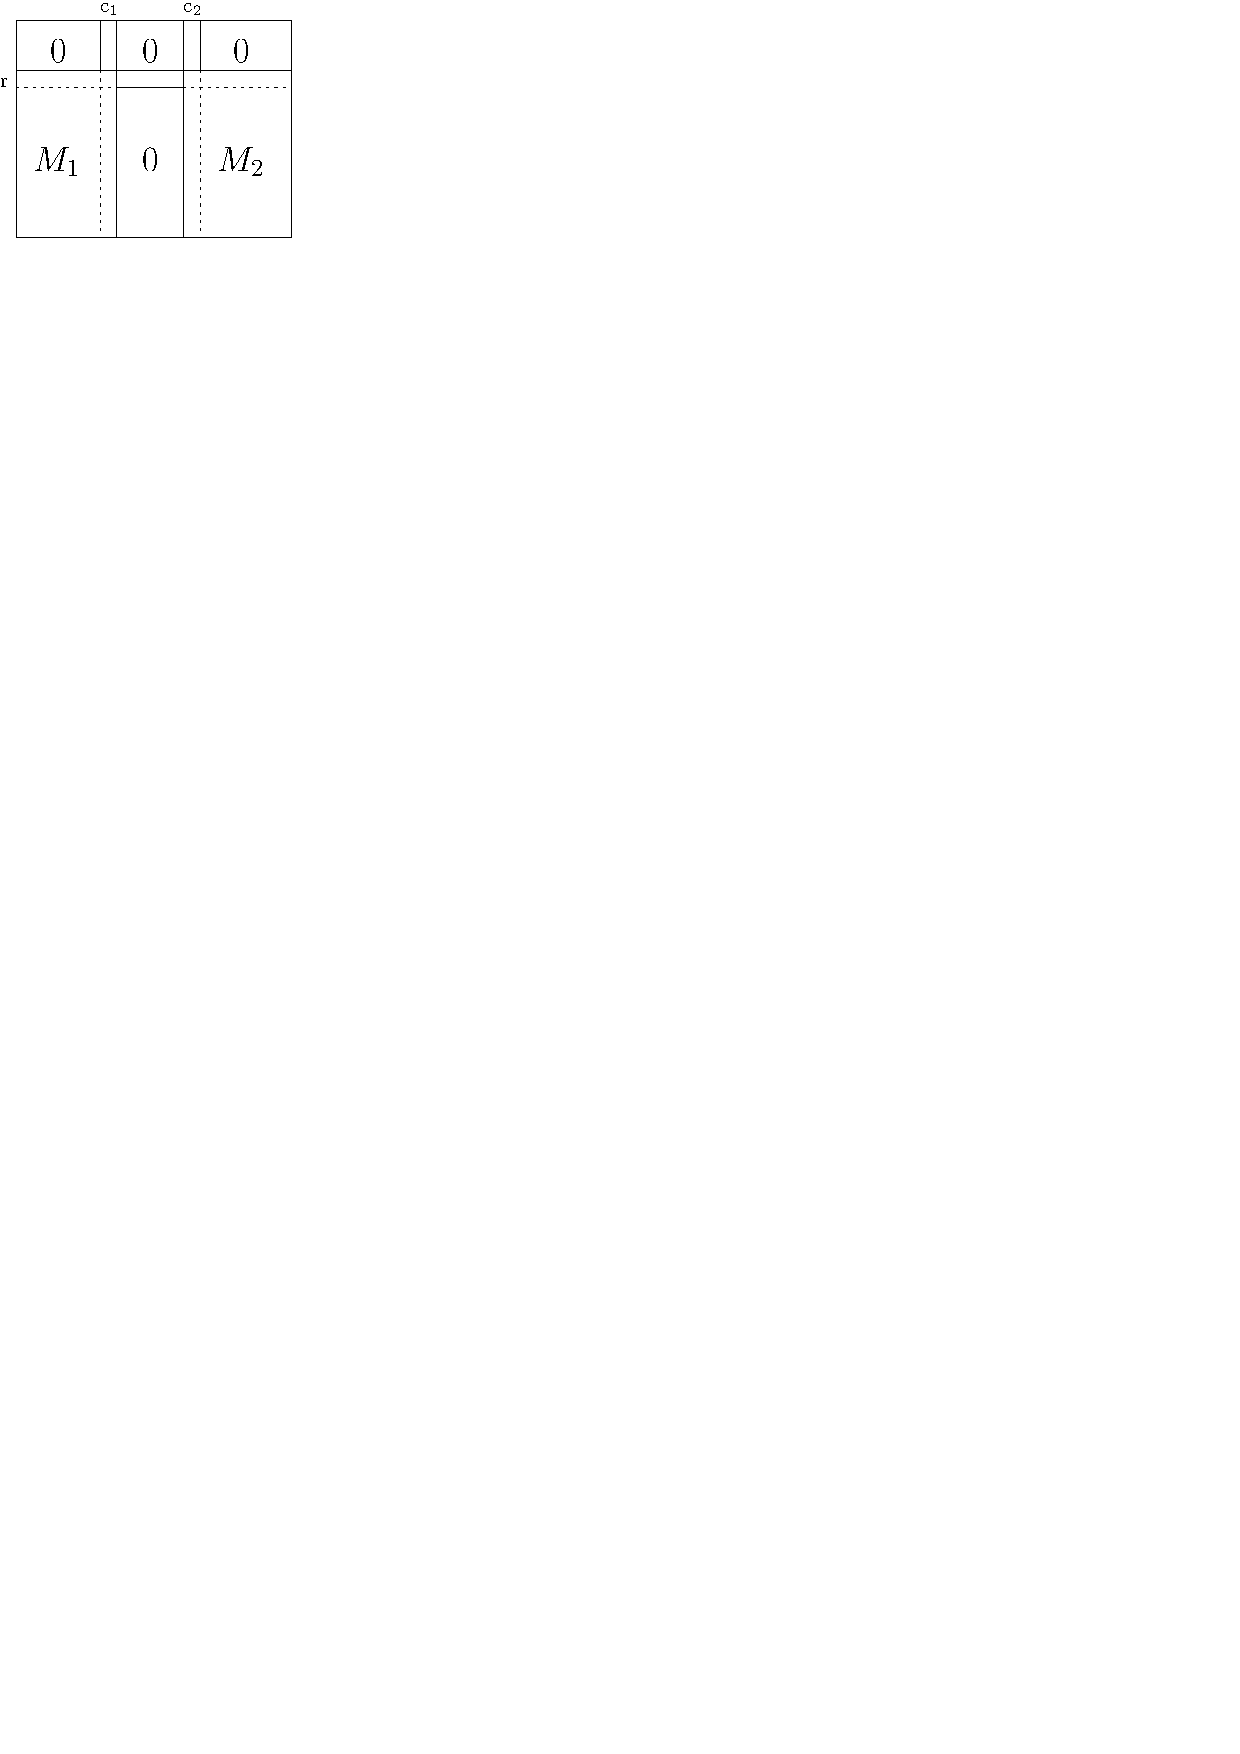
\includegraphics[height=60mm]{img/p72.pdf}
\caption{Characterization of a matrix avoiding \usebox{\smlmatb} as an interval minor.}
\label{p72}
\end{figure}
\begin{proof}
\begin{itemize}
\item[$\Rightarrow$] From Lemma~\ref{lemma2} we know $M=M_1'\oplus_hM_2'$ where $\smm{1&1\\0&1}\nim M_1'$ and $\smm{0&1\\1&0}\nim M_2'$. The second case would be dealt with symmetrically. From Theorem~\ref{theorem1} we have that $M_1'$ can be characterized exactly like $M[[m],[c_2-1]$ and $M[[m],[c_2,n]]$ forms a walking matrix. The only problem with our claim would be if there were two different columns having a one-entry above the $r$-th row. In that case, those two one-entries together with a one-entry in the $r$-th row between the columns $c_1$ and $c_2$ and a one-entry in the $c_1$-th column above the $r$-th row form $P$ as an interval minor.
\item[$\Leftarrow$] The bottom-middle one-entry of $P$ can not be mapped anywhere but to the $r$-th row, but in that case there are at most two columns having one-entries above it. %(will do better hopefully)
\end{itemize}
\end{proof}
\begin{thm}
Let $P=\smm{0&1&1\\1&0&0}$, then for all $M$: $\PnimM\Leftrightarrow M$ contains a walk $w$, no one-entries below the walk and for each entry $M[r,c]$ of the walk there is at most one non-empty column in $M[[r-1],[c+1,n]]$.
\end{thm}
\begin{proof}
\begin{itemize}
\item[$\Rightarrow$] Let $w$ be any walk containing all the top-most and right-most entries that are bottom-left empty. From the choice of $w$, there are no one-entries below it and if all $M[r,c]$, $M[r-1,c]$ and $M[r,c+1]$ are on $w$ then $M[r,c]$ is a one-entry as else $M[r,c]$ was neither top-most nor right-most bottom-left empty. As a consequence, whenever we choose $M[r,c]$ from $w$, it either is a one-entry or there is one-entry in the same row to the left of it. For contradiction let us now assume that there is an entry of the walk $M[r,c]$ for which there are two non-empty columns in $M[[r-1],[c+1,m]]$. Then a one-entry from each of those columns and a one-entry in $M[r,c]$ or to the left of it together give us $\PimM$ and consequently a contradiction. 
\item[$\Leftarrow$] For contradiction let $\PimM$. Without loss of generality we can assume that the bottom-left entry of $P$ is mapped somewhere to the walk -- to $M[r,c]$. But then $\smm{1&1}\im M[[r-1],[c+1,n]]$ which is a contradiction with it having one-entries in at most one column.
\end{itemize}
\end{proof}